%%
%%
%%
%%
%\section{QuickDough}
In short, QuickDough is a nested loop accelerator generation framework that is able to produce hardware accelerators rapidly~\cite{Lin:2012:EDC:2460216.2460227,Liu:2015:FSP}.
Given a user-designated loop for acceleration, QuickDough automatically generates and optimizes the corresponding hardware accelerator and its associated data I/O facilities with the host software (\figref{fig:qd_overview}).



\begin{figure}
\centering
\includegraphics[width=0.9\linewidth]{qd_overview}
\caption{QuickDough takes a user-designated loop as input and generate the corresponding hardware accelerator system using a soft coarse-grained reconfigurable array overlay.}
\label{fig:qd_overview}
\end{figure}

The overall design goal of QuickDough is to enhance designer's productivity by greatly reducing the hardware generation time and by providing automatic optimization of the data I/O between the host software and the accelerator.
Instead of spending hours on conventional hardware implementation tools, QuickDough is capable of producing the targeted hardware-software system in the order of seconds.
By doing so, it provides a rapid development experience that is compatible with that expected by most software programmers.

To achieve this compilation speed, while maintaining a reasonable accelerator performance, QuickDough avoids the creation of custom hardware directly for each application.
Instead, the compute kernel loop bodies are scheduled to execute on a CGRA overlay, which is selected from a library of pre-implemented hardware library.
By sidestepping the time-consuming low-level hardware implementation tool flow, the time to implementing an accelerator in QuickDough is reduced to essentially just the time spent on overlay selection and scheduling compute operations on the resulting overlay.
In addition, taking advantage of the overlay's softness and regularity, QuickDough allows users to perform tradeoff between compilation time and performance by selecting and customizing the overlay on a per application basis.  The result is a unified design framework that seamlessly produces the entire hardware-software infrastructure with a design experience similar to developing conventional software.

Through these facilities and through carefully partitioning the design process, QuickDough strives to improve design productivity of software programmers utilizing FPGA accelerators in 3 aspects:

\begin{enumerate}[nosep]
\item It automates most of the hardware accelerator generation process, requiring only minimum input from the application designer;
\item It produces functional hardware designs at software compilation speed (order of seconds), greatly increasing the number of debug-edit-implement cycles per day achievable;
\item It allows software programmers to progressively improve performance of the generated accelerator through subsequent optimization phases, essentially separating the functional verification and optimization process of application development.
\end{enumerate}

In the following subsections, an overview of QuickDough is presented to illustrate how it achieves the above goals.  For details, please refer to ~\cite{Lin:2012:EDC:2460216.2460227,Liu:2015:FSP}.

\subsection{Generation Framework}
\figref{fig:framework} shows an overview of the QuickDough compilation flow.
The key to rapid accelerator generation in QuickDough is to partition the complex hardware-software compilation flow into a fast and a slow path. 

\begin{figure}
    \center{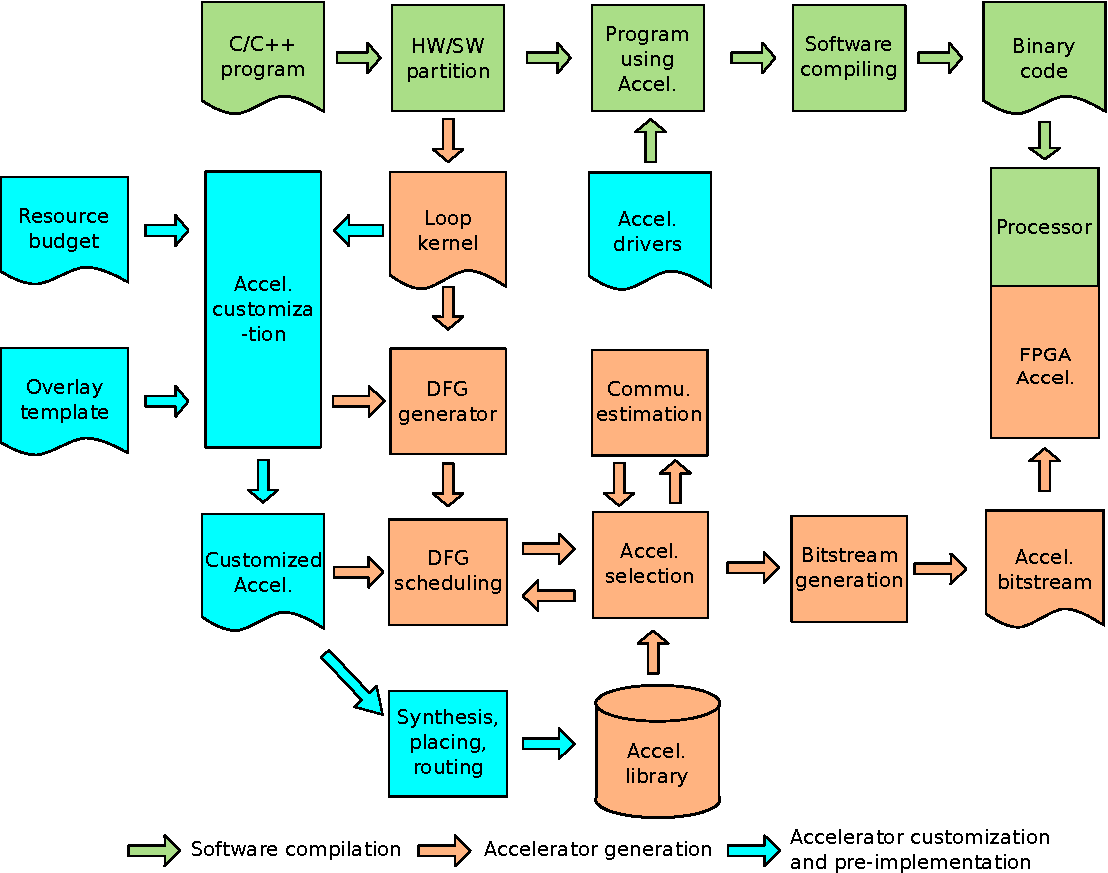
\includegraphics[width=0.8\linewidth]{quickdough_framework}}
    \caption{QuickDough: FPGA loop accelerator design framework using 
        SCGRA overlay. The compute intensive loop kernel of an 
        application is compiled to the SCGRA overlay based FPGA
    accelerator while the rest is compiled to the host processor.}
    \label{fig:framework}
\end{figure}

The fast path of QuickDough consists of the steps necessary to generate a \emph{functional} loop accelerator, which are shown in orange for hardware and in green for software generation in \figref{fig:framework}.
To begin generating a loop accelerator, QuickDough first partially unroll the compute kernel loop and extract the loop body into its corresponding data flow graph (DFG).
Subsequently, a suitable overlay configuration is selected from the pre-built implementation library on which the DFG is scheduled to execute.
Optionally, the user may choose to iteratively refine the selection by feeding back scheduling performance and estimated communication cost at each iteration.
The selected pre-built overlay implementation is then updated with the corresponding scheduling result to create the final FPGA configuration bitstream.
Finally, this updated bitstream is combined with the rest of the software to form the final application that will be executed on the target CPU-FPGA system. 

While there may seem to be a lot of steps involved in this fast path, all of them run relatively quickly.
Furthermore, the only loop in this compilation flow is the accelerator selection process, which as explained is an optional step that can be bypassed if the user opts for speed over quality.
The result is that the run time of this fast path can be kept within the order of tens of seconds.
It allows users to perform rapid design iterations, which is particularly important during early application development phases.

On the other hand, the slow path of QuickDough consists of all the remaining time-consuming steps in the flow from \figref{fig:framework}.
These steps are responsible for implementing the overlay in hardware, optimizing the CGRA to the user application, and updating the overlay library as needed.
Although these steps are slow, they are not necessarily by run for every design compilation.
For example, running through the low-level FPGA implementation is a slow process, however, they are needed only when a new overlay configuration is required.
If a compatible overlay configuration already exists in the pre-built overlay library, then the user may choose to reuse the existing implementation during early developments to facilitate fast design turn-around.
When the user decides that she is ready to spend time optimizing the overlay configuration, she may then instruct QuickDough to execute these slow steps.  With the slower steps, QuickDough will then be able to analyze the user application requirement, customize the overlay accordingly, and finally generate the FPGA configuration bitstream.
Once this bitstream is stored in the overlay library, the user will not need to go through these slow process again.

Throughout the entire application development cycle, most of the time the user will be able to execute only the fast steps, and run through the slow steps only occasionally.
As a result, the overlay compilation speed remains orders of magnitude better than traditional hardware design flow on average.

\subsection{The QuickDough Overlay}
\figref{fig:qd_overlay} shows an overview of the QuickDough overlay together with its data I/O infrastructure.
The QuickDough overlay as shown in the right hand side consists of an array of simple processing elements (PEs) connected by a direct network.
Each PE computes and forwards data to their neighbors synchronously according to a static schedule.
This schedule is stored in the instruction ROM associated with each PE and controls the action of each PE's action in every cycle.
Finally, each PE contains a scratchpad data memory for run-time data that may be reused in the same PE or be forwarded in subsequent steps.

\begin{figure}
    \center{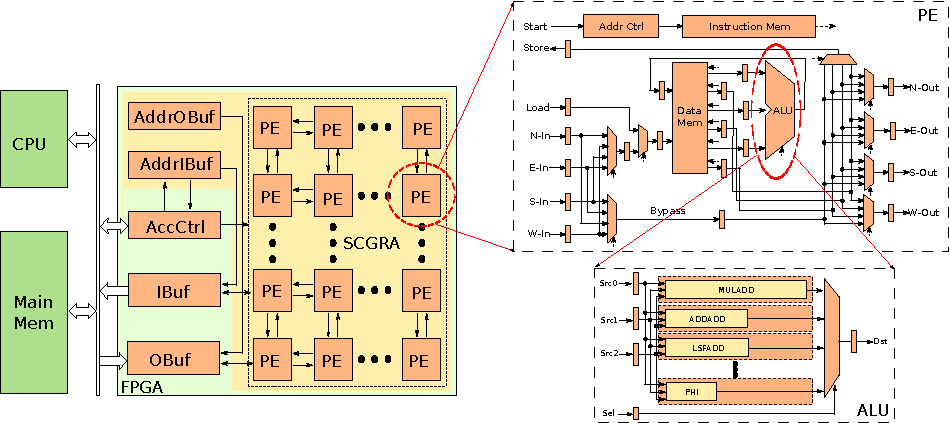
\includegraphics[width=\linewidth]{qd_overlay}}
    \caption{Overview of the QuickDough generated system.  Implemented on the FPGA is the QuickDough overlay, which is an array of PEs connected with a direct network, and the communication infrastructure with the host.}
    \label{fig:qd_overlay}
\end{figure}

Communication between the accelerator and the host processor is carried through a pair of input/output buffers.
Like with the rest of the PE array, accesses to these I/O buffers from the array also take place in lock step with the rest of the system.
The location to access in each cycle is controlled by a pair of address buffers, which contains address information generated from the QuickDough compiler. 

\figref{fig:qd_overlay} also shows the connection within a processing element.
Each PE is constructed surrounding an ALU, with multiplexors connecting the input/output of the ALU to either the internal memory or the neighboring PEs.
In this particular version, the optional load/store path is also shown, which is presented only at dedicated PE connected to the I/O buffer.
Within the PE, the ALU is supported by a multi-port data memory and an instruction memory.
Three of the data memory's read ports are connected to the ALU as inputs, while the remaining ports are sent to the output multiplexors for connection to neighboring PEs and the optional store path to output buffer (\texttt{OBuf}) external to the PE.
At the same time, this data memory takes input from the ALU output, data arriving from neighboring PEs, as well as from the optional loading path from the data input buffer (\texttt{IBuf}).

The ALU itself has a simple design that supports up to 16 fully pipelined operations.
It is constructed also as a template and may be customized to support any user-defined 3-input operations.
Regardless of its function, each operation must have a deterministic pipeline depth.
With that, the QuickDough scheduler will ensure there is never any output conflict and allow the operations to execute in parallel as needed.

Finally, note that the overlay is designed as a soft template.
Many parameters of the overlay, including the SCGRA array size, I/O buffer size, as well as the operations supported by the ALU, are configurable.
They can be optimized for a particular group of application upon user's request as part of the framework's customization steps.






\subsection{Loop Accelerator Generation}
As mentioned, an important goal of QuickDough is to generate high-performance FPGA accelerator systems in software compilation speed.  In this subsection, we will walk through some of the major steps involved and explore the details on how they help generate hardware accelerators very efficiently.


\subsubsection{DFG Generation}
The top-level inputs to QuickDough are loops that the user has designated for acceleration.
To accelerate a loop, the straightforward way is to treat each loop iteration as an individual acceleration target and rely on the host processor for loop control.
However, it is not ideal because (i) the overhead for data and control transfer between the host and FPGA will be too high, (ii) the amount of parallelism encapsulated in a single iteration of the loop body is likely to be too low for acceleration, and (iii) there will be no data reuse between loop iterations to amortize the transfer overhead between the host and the FPGA.

Therefore, just like most other acceleration frameworks, QuickDough begins the accelerator generation process by partially unrolling the input loop $U$ times to increase the amount of parallelism available.
The body of this partially unrolled loop subsequently forms the basic unit $B$ for acceleration in later steps.
This is the unit that is implemented on the FPGA accelerator using the SCGRA overlay.
With a single copy of $B$ implemented in the accelerator, the original loop is completed by executing the accelerator $N/U$ times, where $N$ is the original loop bound.

Furthermore, to amortize the communication cost between the host processor and the accelerator, input/output data are transferred in groups for $G$ invocations unit $B$ as shown in \figref{fig:blocking-and-dfg-gen}.
By buffering I/O and intermediate data on the accelerator, this grouping strategy also allow reusing data between loop iterations, further enhancing performance.

\begin{figure}
\center{\includegraphics[width=0.75\linewidth]{dfg-gen}}
\caption{Loop execution on an SCGRA overlay based FPGA accelerator}
\label{fig:blocking-and-dfg-gen}
\end{figure}

In our current implementation, the unrolling factor $U$ is specified by the user, while the grouping factor $G$ is determined by the framework automatically.
$G$ is determined based the on-chip buffer size

At the end of this process, the unrolled loop body $B$ will form the core of the accelerator and the corresponding data flow graph (DFG) will be extracted, which will drive the rest of the generation flow.



\subsubsection{Accelerator Selection}
As an accelerator generation framework, an important task of QuickDough is without doubt to generate the physical implementation of the accelerator on the FPGA.
With its SCGRA serving as an intermediate layer, this translates into physically implementing the overlay on the FPGA.
Unfortunately, no matter how simple the overlay is, running through the low-level hardware implementation tools is going to be a lengthy process, contradicting the original goal of employing the overlay in the first place.
In order to sidestep this lengthy hardware implementation process, QuickDough instead transform it into a selection process from a library of pre-implemented overlay.

When compared to directly implementing the overlay using standard hardware implementation tools, this accelerator selection process is much faster.
In return, the performance of the resulting overlay configuration may not be optimal for the given user application.
Despite the suboptimal performance, the selected overlay implementation is functionally correct and should give a good sense of the overall hardware-software codesign process to the software programmer, which is necessary for rapid early development.
The user may subsequently opt for the slower optimization and customization steps explained in the next subsection to progressively improve performance.

As such, the goal of this process is to select the \emph{best} and \emph{functional} overlay configuration from the pre-implemented library \emph{rapidly}.
While functionality is easy to determine, QuickDough must also be able to estimate the resulting performance swiftly for this selection process.
Now, the performance of the accelerator depends mainly on two factors: (i) computational latency, and (ii) communication latency.
As the SCGRA overlay is regular and computes with a deterministic schedule, its exact computational latency of carrying out the user DFG can readily be obtained from the scheduler.
Of all the configurable parameters of the overlay, the SCGRA array size is the dominant factor affecting this computational latency.
On the other hand, communication latency depends not only on the scheduling results, but also other factors such as communication pattern, grouping factor, I/O buffer sizes, as well as DMA transfer latency, etc.
These parameters interact with each other to form a large design space.
For rapid estimation, instead of performing a full design space exploration, QuickDough is able to rely on simple analytical model for estimating communication latency based on the overlay SCGRA array size.

Finally, QuickDough leaves this choice of effort in finding the best accelerator configuration to the user as 3 optimization effort levels:
\begin{itemize}[nosep]
\item Level 0 (\texttt{O0}) -- No optimization.  QuickDough selects a feasible accelerator configuration with the smallest SCGRA size.
\item Level 1 (\texttt{O1}) -- QuickDough estimates performances of 3 accelerators with different array sizes and select the one that results in the best performance.
\item Level 2 (\texttt{O2}) -- QuickDough performs an exhaustive search on all accelerators in the library and searches for the best accelerator configuration. 
\end{itemize}

Obviously, the more effort is being put into the selection process, the longer the process will take, and the resulting performance is improved most of the time.
The choice on how much effort to pay is up to the user.

\subsubsection{DFG Scheduling}
This is the step where the DFG extracted from the unrolled loop body is scheduled to execute on the selected SCGRA overlay.
For each operation in the DFG, the scheduler must decide the cycle and the PE in which the operation should be carried out.
The scheduler also determines the routing of data between the producing and consuming PEs, as well as to/from the I/O buffer.

As QuickDough tends to target DFGs with close to thousands of node, to keep the scheduling time short, a classical list scheduling algorithm was adopted~\cite{schutten1996list}.
A scheduling metric proposed in~\cite{Lin:2012:EDC:2460216.2460227} that considers both load balancing and communication cost was used in the scheduler.

At the end of this scheduling step, a schedule with operation of each PE and data I/O buffer in every cycle is produced.
This schedule essentially turns the generic overlay implementation into the specific accelerator for the user application.


\subsubsection{Accelerator Bitstream Generation}
The final step of the accelerator generation process is to produce the instructions for each PE and the address sequences for the I/O buffers according to the scheduler's result.

As a way to reduce area overhead of the overlay, both the instruction memory of each PE as well as the I/O address buffers are implemented as read-only memories (ROMs) on the physical FPGA.
To update the content of these memories, the QuickDough framework must update the FPGA implementation bitstream directly.
%
To do that, the memory organization and placement information of the target overlay implementation is obtained from an \code{XDL} file corresponding to the overlay implementation \cite{beckhoff2011xilinx}.
The resulting memory organization information is encoded in the corresponding \code{BMM} file, which is combined with the scheduler results to update the overlay implementation bitstream with the the \code{data2mem} tool from Xilinx \cite{data2mem}.

While it may sound complicated, the whole process is automated and consumes only a few seconds of tools run time.
The result of this process is an updated bitstream with all application-specific instructions embedded.
This updated bitstream is the final configuration file used to program the physical FPGA, and it concludes the QuickDough flow.


\subsection{Customization \& Optimization}
The true power of utilizing an FPGA overlay rests on that fact that the overlay is virtual, soft, and easily customizable for the need of the application.
In this part, we will examine various ways QuickDough enables user to customize and optimize the overlay to improve power-performance of the generated accelerators.
Unlike the fast generation path explained above, these customization steps are much more time consuming.
As such, these customization steps are considered part of the slow path in QuickDough's design philosophy, and are expected to execute only occasionally as needed.

There are a number of reasons why a user may want to spend the time on customization despite the slow process.
To begin, the user may want to construct a prebuilt implementation library specific to the target application domain. 
It is useful as the result can be memoized in the implementation library and be reused by all other target applications, amortizing the initial implementation effort.
Once the project development has gone through the initial debugging phase, a user may also opt for creating a customized overlay for the particular accelerated application.
This per-application optimization will help improve the performance of the accelerator but the process will undoubtedly be slower than to select a prebuilt implementation.
Luckily, the result of this per-application customization can be stored in the prebuilt library such that it can be reused on subsequent compilations.

\subsubsection{What can be customized?}
For the purpose of customization, the QuickDough overlay was designed from the beginning to be a template from which a family of overlay instances could be generated.
The SCGRA overlay consists of a regular array of simple PEs connected with direct connections.
Depending on the application requirements, a range of design parameters of this overlay can then be customized, including the array size, on-chip scratchpad data memory capacity, instruction memory capacity and I/O buffer capacity.
On top of that, as a hardware-software system generator for loop acceleration, QuickDough may also optimizes the communication between the accelerator and the host software by varying the \emph{grouping factor}, which determines the amount of data transferred between the two in each transaction.
Finally, it may also optionally optimizes the \emph{loop unrolling factor} on behalf of the user depending on the computational capability of the overlay as a function of its array size.

Obviously, a major challenge when optimizing this set of parameters is that they tend to interact with one another in fairly complex ways.
For example, increasing the array size increases the compute capability of the array, potentially improving the accelerator performance.  However, the increased size is beneficial only if the input DFG has enough parallelism presented to take advantage of the increased capability.
To increase the amount of available computation, QuickDough may optionally increase the amount of loop unrolling in the user-supplied kernel.
However, that also increases the amount of data I/O required, as well as the on-chip instruction and data buffer requirement, which in turn limits the size of the array in the first place.
A full discussion of the detailed customization and optimization process is beyond the scope of this chapter.  Yet it is worthwhile to realize the potential of customization here.

As an illustration, \figref{fig:qd_customization_fir} shows the effect of customization on the generated accelerators from QuickDough.
In this example, accelerator for a 49-tap FIR filter was generated on the Zedboard using QuickDough.
Three different customized overlay configurations were generated.
Beginning with the specified array size, the rest of the configuration parameters were determined automatically. 


\begin{figure}
\centering
\subfigure[Performance]{
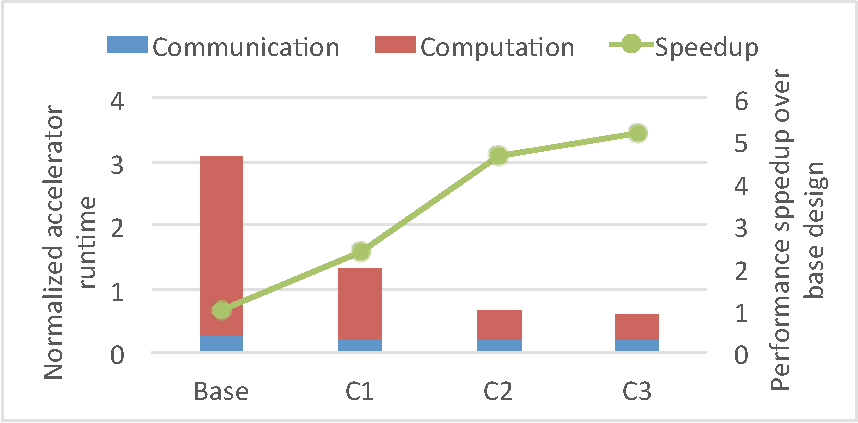
\includegraphics[width=0.47\linewidth]{qd_customization_ex}
\label{fig:qd_customization_ex}
}
\hfill
\subfigure[Resource Consumptions]{
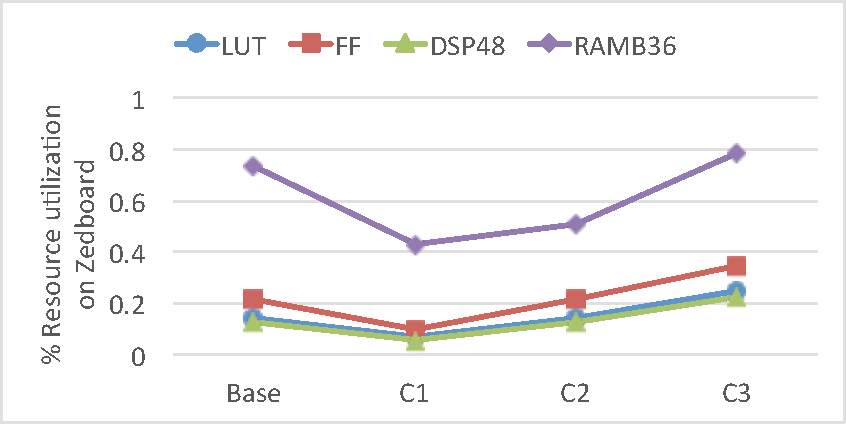
\includegraphics[width=0.47\linewidth]{qd_customization_resource}
\label{fig:qd_customization_resource}
}
\newline
\subfigure[Overlay configuration]{
\begin{minipage}{0.9\linewidth}
\centering
\footnotesize
\begin{tabular}{ccccc}
\toprule
&base&C1&C2&C3\\
\midrule
Loop unrolling factor&10$\times$50&50$\times$50&50$\times$50&50$\times$50\\
Grouping factor&100$\times$50&2500$\times$50&1250$\times$50&5000$\times$50\\
SCGRA size&3$\times$3&2$\times$2&3$\times$3&4$\times$4\\
Inst Mem Depth&4k&4k&2k&1k\\
IO Buffer Depth&1k&4k&2k&8k\\
\bottomrule
\end{tabular}
\end{minipage}
}
\caption{Effect of overlay customization on performance and resource consumption.  Example here shows the result of an FIR filter using QuickDough with 3 different overlay configurations over a base design.}
\label{fig:qd_customization_fir}
\end{figure}

A few interesting observations can be made from the figures.  In terms of performance, comparing to the sub-optimal baseline configuration, the best configuration (\textsc{c3}) results in more than 5 times improvement in performance.
Furthermore, comparing the baseline and \textsc{c2} that feature the same array size ($3\times 3$), $4.7\times$ improvement in performance can be obtained by optimizing the unrolling and grouping factor in combination with the on-chip memory configuration.
Interestingly, looking at the resource consumptions, \textsc{c2} in fact consumes $31\%$ less on-chip memory and the same resource otherwise as the baseline.

\subsection{Summary}
Using QuickDough as a case study, we have illustrated how the use of an FPGA overlay has enabled a very different experience for software programmers when designing hardware-software systems.
The 2-layer approach to hardware design allows for a very rapid design experience that sharply contrasts the lengthy low-level hardware tool flow.
Furthermore, the softness of the overlay provides opportunity for further customization and optimization as the development effort progresses.
Together, it creates for novice users a ``software-like'' way to designing complex accelerator systems while maintaining considerable overall acceleration performance promised by FPGAs.



%%
%%
%%
%%

